\href{https://github.com/yassienE4/OS-Portfoilio/commit/2472c7bcc4ca4e584a5f7c1c9ceb7fcce6b61607}{\ul{https://github.com/yassienE4/OS-Portfoilio/commit/2472c7bcc4ca4e584a5f7c1c9ceb7fcce6b61607}}

How to run

\begin{itemize}
\item
  Verify openssl is installed, openssl version
\end{itemize}

\begin{itemize}
\item
  Go to working directory, cd passwords
\item
  Compile, g++ main.cpp -o main -lssl -lcrypto
\item
  Run, ./main
\end{itemize}

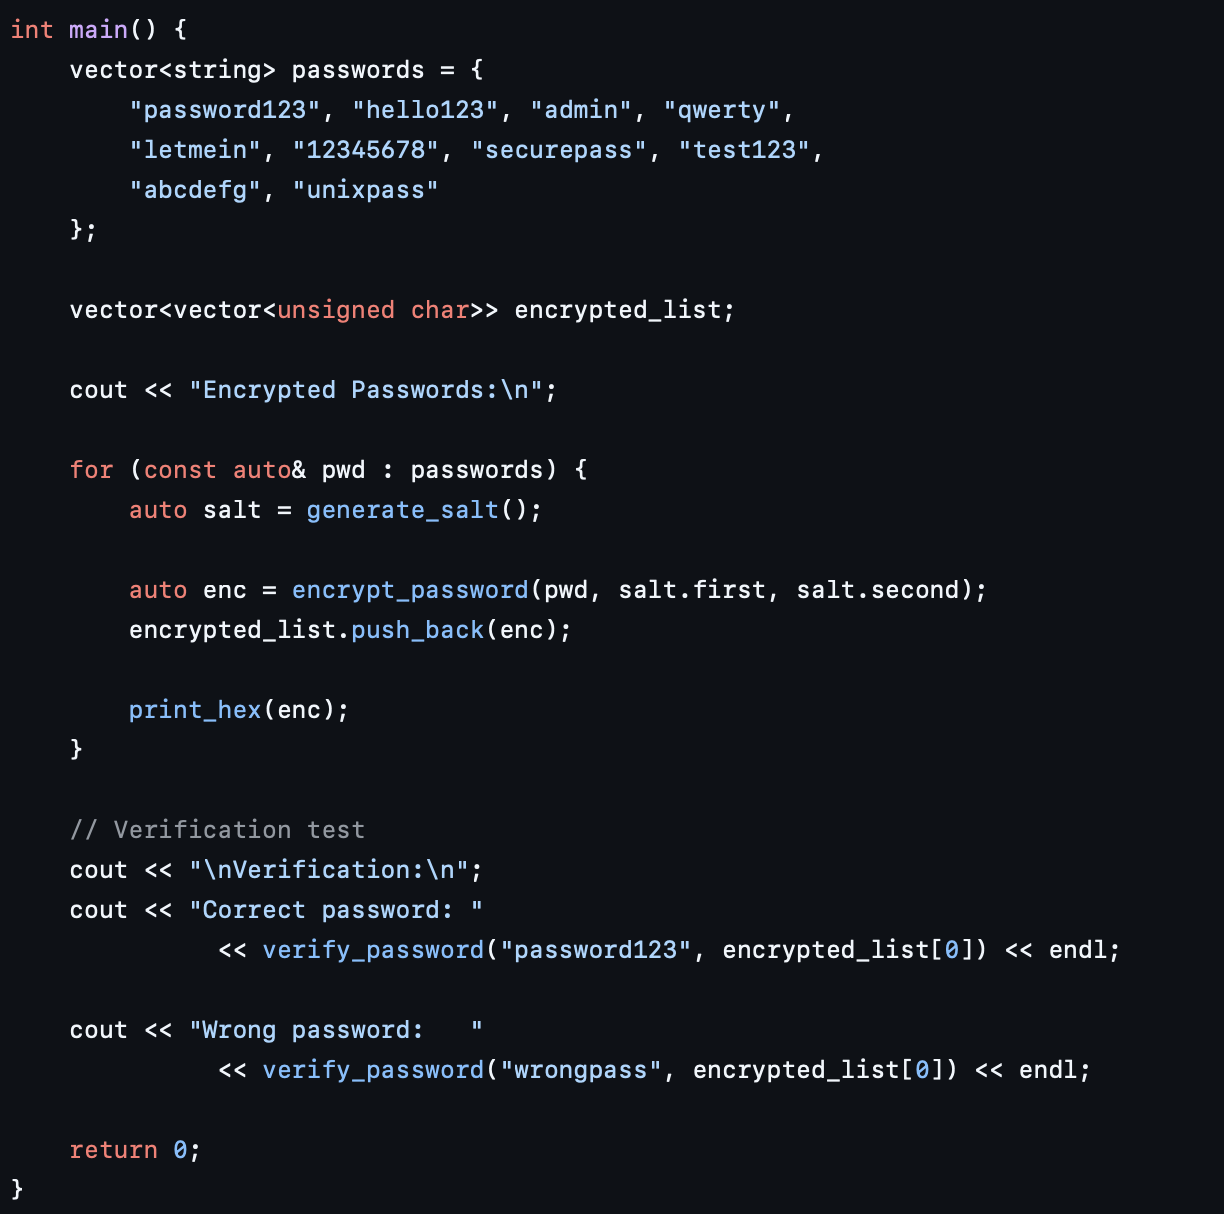
\includegraphics[width=5.11746in,height=5.07646in]{./images/media/image3.png}

First I create a list of 10 passwords, and an empty list to store the
encrypted passwords

For every password i create unique salt, and then encrypt the password
using the salt, before adding it into the list,

To verify i pass the correct the password, and it reapplies the
algorithm to get a new encrypted password which it checks against the
stored password

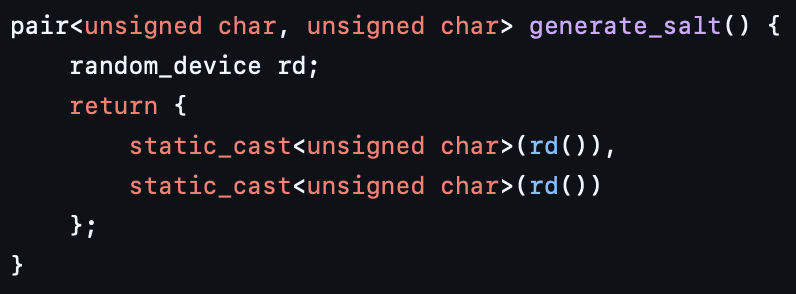
\includegraphics[width=4.74479in,height=1.75649in]{./images/media/image1.png}

To generate a salt, i just create 2 random 8 bit strings, so that i can
have a 16 bit string

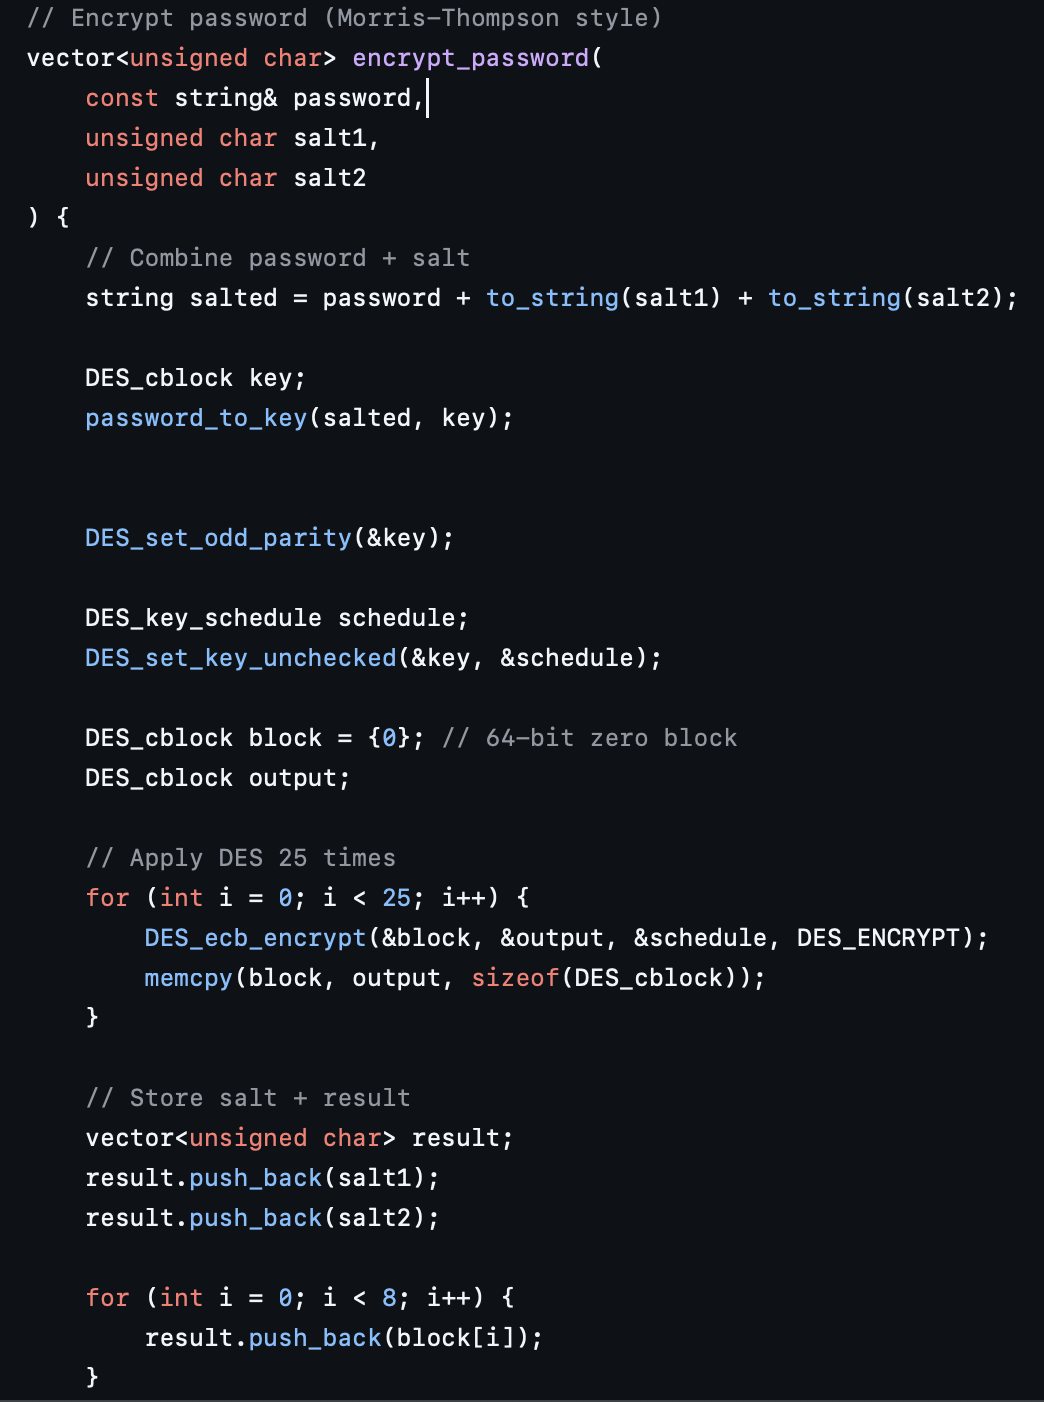
\includegraphics[width=4.18967in,height=5.61979in]{./images/media/image4.png}

To encrypt the password first I add the salt to the password, then I
convert the password to an 8 byte des key, which I use to apply the DES
algorithm 25 times. I then store both the encrypted password and the
salt in the final array.

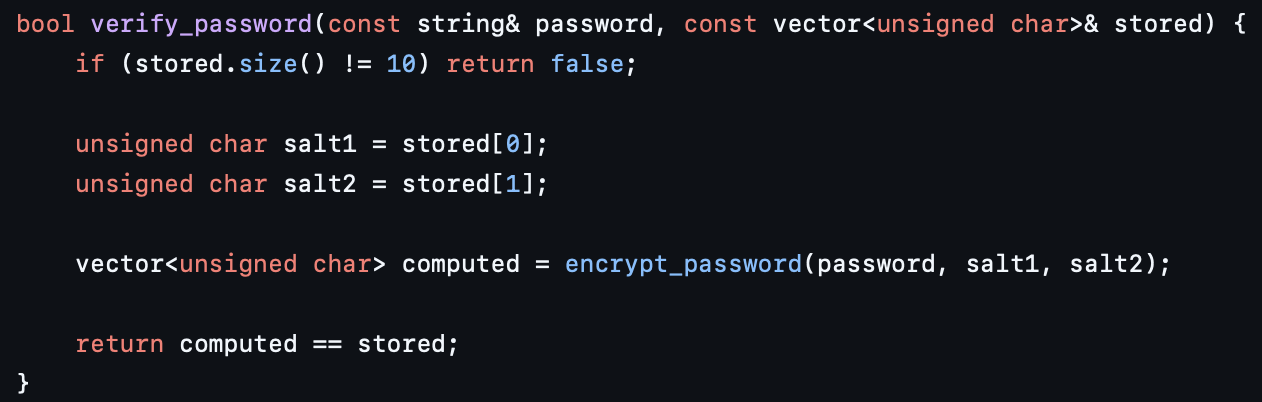
\includegraphics[width=6.5in,height=2.06944in]{./images/media/image2.png}

To verify a password, i first have to retrieve the salts stored, so that
i can compute a new encrypted password using the same salts,

I then compare the computed password with the stored to verify.

And return the result.
